\documentclass[12pt]{article}
\usepackage[utf8]{inputenc}
\usepackage{amsmath}
\usepackage{amssymb}
\usepackage{graphicx}
\usepackage{algpseudocode}

\graphicspath{ {./} }

\newcommand{\rectres}[1]{
\begin{center}
\begin{tabular}{ |c| }
\hline\\
#1\\
\\
\hline
\end{tabular}
\end{center}
}

\newcommand{\qed}{\hfill$\blacksquare$}

\title{Introduction to AI - 236501\\HW1}
\author{Yair Nahum 034462796\\and\\Hala Awwad 209419134 }

\begin{document}

\maketitle

%\tableofcontents{}

\section{Intro}

\subsection{}
We use the notation as in the tutorial about the sets as follows:\\
$$[n] \equiv \{ 1,2,...,n\}$$
Next, we define the $\{S,O,I,G\}$ as follows:\\
For the states we know we have 25 places for the taxi to be in the grid.\\
We have 5 states for the passenger to be $\{R,Y,G,B\}\cup\{in the taxi\}$.
and 4 states for the destination $\{R,Y,G,B\}$.\\
Thus, 
$$S = [500] \Rightarrow $$
$$ |S| = 25*5*4 = 500$$
The valid states as defined in the hw notebook are a subset of this states space as the passenger and destination are not at the same location (3 options are left to seleect from for the destination). So,\\
$$ |S| = 25*5*3 = 375$$
The operations/actions that our taxi agent can perform are:\\
$$O = \{0="South",1="North",2="West",3="East",4="Pickup",5="Dropoff"\}\Rightarrow$$
$$|O| = 6$$
The initial states can be random, but as defined in the hw notebook, we always starts at $s = 328$. Thus,\\
$$I=\{328\}\Rightarrow |I|=1$$
The goal state is when the taxi and passenger are at the destination after the passenger was dropped there. So we have 4 different goal states:\\

$$G=\{s\in S | \{Taxi\wedge Passenger \wedge Destination\in R\} \cup $$
$$\{Taxi\wedge Passenger \wedge Destination\in Y\} \cup $$
$$\{Taxi\wedge Passenger \wedge Destination\in G\} \cup $$
$$\{Taxi\wedge Passenger \wedge Destination\in B\} \} \Rightarrow$$
$$|G|=4$$
\subsection{}
The Domain of the "North" operation are all the states.\\
There are states in which the taxi will stay at the same state if it goes north.\\
More formally:
$$Domain(o_1="North")\equiv\{s\in S | o_1(s)\neq \phi\} = S$$
One can think that it's illegal to go north on the top row of the grid world or when  there are horizontal walls north to a reachable grid cell. But the env allows the taxi to go north with reward -1.
More formally, if it was illegal:\\
$$Domain(o_1="North")\equiv\{s\in S | o_1(s)\neq \phi\} = $$
$$\{s\in S |s\in \{\text{All states in which the taxi is not at the north-est grid row} \}\}$$

\subsection{}
The function Succ over the initial state 328 will return all the neighbors of that state, and as we got from running getNeigbours on the initial state\\
$$South(328)=428$$
$$North(328)=228$$
$$East(328)=348$$
On West/Dropof/Pickup operation we stay at the same location (there is a wall to the west):
$$West(328)=Pickup(328)=Dropoff(328)=328$$
More formally:
$$Succ(s=328)\equiv\{s'\in S | \exists o\in O, s.t. [s \in Domain(o)\wedge o(s)=s'\} = $$
$$\{428,228,348,328\}$$
\subsection{}
for the worst case, we can randomly switch between several cases and never reach a destination. so for the random agent we can get infinite number of actions for the agent.\\
Since the state space is finite, and there is an equal probability for each action, the agent eventually will find the goal (finite MDP with positive probability and we can compute the expectation for reaching the goal).
\subsection{}
If the agent does the optimal actions by chance, we can see the optimal path is:\\
1. 4 actions to reach the passenger (North,West,South,South)\\
2. 1 action to Pickup\\
3. 4 North actions\\
4. 1 action to Dropoff\\
Therefore, we have total of 10 actions at the optimal path.
\subsection{}
As we wrote on the previous section, the optimal path is:
(North, North, West, South, South, Pickup, North, North, North, North, Dropoff)
The rewards are therefore:\\
(-1, -1, -1, -1, -1, -1, -1, -1, -1, 20)
And the total reward is:
$$\text{total reward} = 9*(-1) + 20 = 11$$

\subsection{}
Yes. There are circles in our search space (if we don't do some graph search that denotes already visited states).\\
For example the following path will get us back to our initial path:\\
(North,East,South,West)\\
If our algorithms of search will maintain the CLOSE lookup table, we can easily check for such circles.

\section{BFS-G}

\subsection{}
We've implemented the BFS-G in code (not tree search).\\
That is, Besides the frontier (the OPEN queue implemented with python list), we maintain a set of states that were already reached (the CLOSE set as described in the book).\\
We've optimized the number of nodes created when expanding some node in the frontier by checking if its neighbor state was already reached or in frontier.\\
A helper set of frontier (OPEN) states was added, although we could check existence of the node in nodes queue (for simplicity of checking vs reached/frontier states' sets)
We've added also some counters for the created and expanded nodes through the search.\\

\subsection{}
The amount of states expanded were 31.\\
BTW, the amount of created nodes was 36 (about 5 nodes remained in the frontier)\\

\subsection{}
This is the same as previous section as we've optimized to create only none reached (not in CLOSE set) and none frontier (OPEN) states.

\subsection{}
The main advantage of the BFS/BFS-G compared to DFS (tree search) is that it's a complete (guaranteed to find a path to the goal) and optimal (that path is the optimal path to the goal state), while DFS (tree search) isn't as it may stuck in infinite loops repeating the same states.\\

In our taxi env, the state space is finite, so if we use DFS-G with graph search (next section), we will find a solution but it may not be optimal.\\

The disadvantage of BFS is its memory consumption which is $O(b^d)$ while the DFS-G $O(bD)$ (with backtracking $O(D)$) When D is the max depth of the taxi env when we start from some state (bounded by the state space size). DFS with tree search may not end and have an infinite memory consumption as we can repeat the same state in the tree (circles). One can run DFS-G or add some circles detection mechanisms (going back several parent nodes for example) as described in the course book.

\subsection{}
Yes. In the taxi environment it will always find the optimal solution, as we saw in the lecture,\\

BFS finds the shortest path (number of edges) to any state in the env.\\
In our case, the taxi env, the edges (actions) doesn't have the same cost but we will still find the optimal solution as the shortest path in edges is also the shortest path in cost.
\subsubsection*{Proof}
Completeness: Assuming a solution of cost (depth) d exists. BFS will return the solution before exposing the d+1 layer, We know it will reach the d+1 layer as it works in layers and we can by induction prove that it finds all the nodes in the next layer.
Optimal: Assume that a solution of cost (depth) d exists and the BFS returns a none optimal solution of cost d’ > d. It will return the optimal solution before exposing the d+1 layer so we get a contradiction.

\section{DFS}

\subsection{}
We've implemented the DFS-G similar to BFS-G but the strategy to pop from the frontier (OPEN) was based on LIFO (stack) and not FIFO(queue) as in BFS.\\
Initially, we've implemented a tree search in which the algo got into infinite loops since we didn't check vs reached states (CLOSE).\\
We've also played with the tie breaking between neighbor nodes (by random shuffle) or by just reversing the order of addition to frontier and got different paths.\\
This is not surprising, as DFS-G may return some solution which is not optimal.
Again, DFS-G \textbf{\emph{on finite state space}} , as in the taxi world, is a complete search algorithm (DFS tree search is not since we can get stuck in a loop) but not optimal. 

\subsection{}
The number of states expanded when we didn't find the optimal path were 96.

\subsection{}
Since we expand only different states as we run DFS-G, the number of states expanded is the same.

\section{ID-DFS}
\subsection{}
Implemented the ID-DFS by calling DFS-L with increasing depth starting from 0 depth.

\subsection{}
We got that the total expanded nodes (sum of all nodes expanded in all depths runs) is 186.\\
This is the summation of the following list which stands for number of expanded nodes in each ID-DFS iteration (increasing depth):\\
expanded\_nodes = [1, 4, 8, 13, 19, 24, 27, 28, 30, 32]

\subsection{}
As we repeat the same expanded nodes when we increase the depth (and add more new states we didn't reach at the max depth), the amount of different states developed is actually the last iteration expanded nodes calculation. In our environment and start state, as we saw on previous section, these are 32 different states.

\subsection{}
The ID-DFS advantage compared to DFS-G is that it's complete and admissible, while DFS-G on finite state space is only complete.\\
The disadvantage of ID-DFS is that it expands the same nodes multiple time and not just once as in DFS-G.

\subsection{}
The advantage of ID-DFS compared to BFS is its memory complexity. In ID-DFS we have $O(bD)$ (b - branching factor, D - is maximal depth from start state as we run DFS-G on finite state space), while in BFS it's $O(b^d)$ (d - optimal path depth).\\
The disadvantage of ID-DFS compared to BFS-G is that it expands the same nodes several times while BFS-G expands each node only once.

\subsection{}
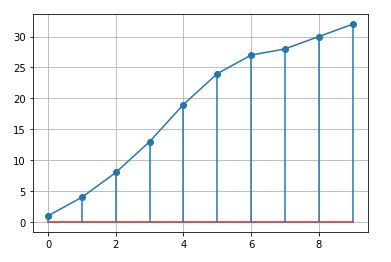
\includegraphics[scale=1]{id_dfs_plot.JPG}\\
We can see from the graph above that as the depth increases the amount of expanded nodes increases as we go deeper at each iteration of ID-DFS and expand states we haven't visited before due to limited depth.

\section{W-A*}
\subsection{}
Implemented the W-A* in code.\\
When w=0.5, we get the A* search.
\subsection{}
Yes. we can expand a reached state (after it's in the CLOSE set) and re-add it to OPEN and expand again:\\
\begin{algorithmic}
\If{s not in OPEN and not in CLOSE}\\
    ...
\ElsIf {s in OPEN}\\
    ...
\Else \Comment{s in CLOSED}\\
    \If{$new\_g <  n\_curr.g()$}
        \State n\_curr \gets update\_node(s, n, new\_g ,new\_g + h(s))\\
        \State OPEN.insert(n\_curr)
        \State CLOSED.remove(n\_curr)
    \EndIf
\EndIf 
\end{algorithmic}
As shown in pseudo code above, when the next state (neighbor of the now expanded node) is already in CLOSE set we $\textbb{update}$ it's f value and re-add it to the OPEN set.
BTW, In case it's in OPEN we also update it.

\subsection{}
When called with the null heuristic we get the UCS solution with 34 states expanded with the optimal cost (10 actions as before, with total reward of 11).

\subsection{}
The optimal cost defined (as was defined in BFS) is the smallest amount of actions to take from start state to goal state. We define the cost of each action as 1.\\
The first 2 heuristics are admissible while the last 2 are not.\\
1. $\textbb{Greedy}$:\\
Since our closest state before the goal is the state just before we drop the passenger at its destination (and thus with the smallest cost as we defined it).\\
We get $\forall s\in S, s \neq goal\_state$ we have $1 \leq h^*(s) = g(s)$\\
Thus, the Greedy heuristic is admissible as $h(goal\_state) = 0$ and $\forall s\in S, s \neq goal\_state$  we have $h(s) \leq h^*(s) = g(s)$. 

\subsection{}
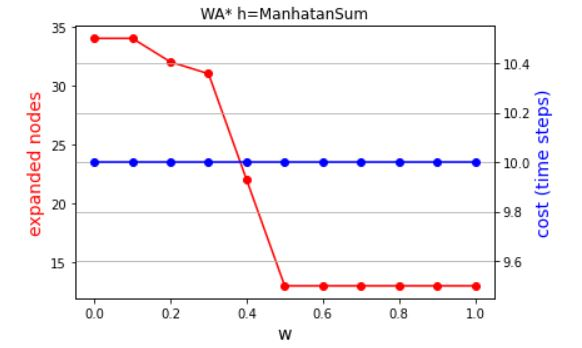
\includegraphics[scale=1]{w_graph.JPG}\\
\end{document}

